\documentclass[12pt, letterpaper]{article}
\usepackage{listings}
\usepackage{graphicx}
\usepackage{color}
\usepackage{caption}
\usepackage{subcaption}
\usepackage{hyperref}
\usepackage{fancyhdr}
\usepackage{mathrsfs}
\usepackage[margin=3cm]{geometry}
\usepackage[dvips]{epsfig}
\usepackage{placeins}
\usepackage{longtable}
\usepackage{wrapfig}
\usepackage{caption}
\usepackage{alltt}

\setlength{\parindent}{0.0in}
\setlength{\parskip}{0.05in}

\definecolor{dkgreen}{rgb}{0,0.6,0}
\definecolor{gray}{rgb}{0.5,0.5,0.5}
\definecolor{mauve}{rgb}{0.58,0,0.82}
\definecolor{deepblue}{rgb}{0,0,0.7}
\definecolor{deepred}{rgb}{0.6,0,0}
\definecolor{deepgreen}{rgb}{0,0.5,0}
\definecolor{red}{rgb}{0.9,0,0}

\newcommand\course{CS532}
\newcommand\semester{Spring 2017}
\newcommand\hwnum{8}
\newcommand\yourname{Justin Schaffner}
\newcommand\login{JASchaff}
\newenvironment{answer}[1]{\subsection*{Problem #1}}

\pagestyle{fancyplain}
\headheight 40pt
\lhead{\yourname\ (\login)\\\course\ --- \semester}
\chead{\textbf{\Large Assignment \hwnum}}
\rhead{\today}
\headsep 40pt

\DeclareCaptionFont{white}{\color{white}}
\DeclareCaptionFormat{listing}{\colorbox[cmyk]{0.43, 0.35, 0.35,0.01}{\parbox{\dimexpr\textwidth-2\fboxsep\relax}{#1#2#3}}}
\captionsetup[lstlisting]{format=listing,labelfont=white,textfont=white, singlelinecheck=false, margin=0pt, font={bf,footnotesize}}
\captionsetup[figure]{format=listing,labelfont=white,textfont=white, singlelinecheck=false, margin=0pt, font={bf,footnotesize}}
\captionsetup[alltt]{format=listing,labelfont=white,textfont=white, singlelinecheck=false, margin=0pt, font={bf,footnotesize}}



\lstnewenvironment{MyBash}[1][]{\noindent\lstset{#1, language=bash, aboveskip=3mm, belowskip=3mm, showstringspaces=false, columns=flexible, basicstyle={\small\ttfamily}, numbers=none, numberstyle=\tiny\color{grey}, keywordstyle=\color{black}, commentstyle=\color{dkgreen}, stringstyle=\color{black}, breaklines=true, breakatwhitespace=true, tabsize=3, frame=tb }}{}
\lstnewenvironment{MyPython}[1][]{\noindent\lstset{#1, language=Python, aboveskip=3mm, belowskip=3mm, basicstyle=\small, otherkeywords={self}, keywordstyle=\color{deepblue}, emph={MyClass,__init__}, emphstyle=\color{deepred}, stringstyle=\color{deepgreen}, commentstyle=\color{red}, frame=tb, showstringspaces=false, breaklines=true }}{}
\lstnewenvironment{MyR}[1][]{\noindent\lstset{#1, language=R, aboveskip=3mm, belowskip=3mm, basicstyle=\small, breaklines=true, frame=tb}}{}

\begin{document}

\begin{answer}{1: Blog Term Matrix}
Question 1: Create a blog-term matrix. Start by grabbing 100 blogs; include:
http://f-measure.blogspot.com/
http://ws-dl.blogspot.com/
and grab 98 more as per the method shown in class. Note that this method randomly chooses blogs and each student will separately do this process, so it is unlikely that these 98 blogs will be shared among students. In other words, no sharing of blog data. Upload to github your code for grabbing the blogs and provide a list of blog URIs, both in the report and in github. Use the blog title as the identifier for each blog (and row of the matrix). Use the terms from every item/title (RSS) or entry/title (Atom) for the columns of the matrix. The values are the frequency of occurrence. Essentially you are replicating the format of the "blogdata.txt" file included with the PCI book code. Limit the number of terms to the most "popular" (i.e., frequent) 1000 terms, this is *after* the criteria on p. 32 (slide 7) has been satisfied. Remember that blogs are paginated.

To grab the 100 blogs one function was created and added to the file ``sevenhtml.py". This file will include all of the functions used for Assignment 7. The function\\ ``get\textunderscore random\textunderscore blog()" shown in Listing \ref{lst:getrandom} takes one argument, which is the language preference for the request header. Whether or not this works perfectly is hard to say, one of the returned blogs did have a title in Cyrillic, but none of the words in the final list appeared to be in another language. The function checks the returned random url for an RSS hyperlink, and if it finds one, it returns it. The script to run this function can be scene in Listing \ref{lst:blogsearch}. It collects 125 unique blog urls and saves them to the file ``lurl.txt" shown at the end of the report.\\
 
Using the functions described in Chapter 2 of Programming Collective Intelligence by Toby Segaran, grabbing the words from the blogs was fairly simple. The function ``getwordcounts()" was modified to support pagination, as shown in Listing \ref{lst:getwordcounts}. The file ``generateFeedVector.py" from the book was modified to handle cases where the title of a blog was not referenced normally, causing a key error when ``getwordcounts()" is called. ``generateFeedVector.py" is shown in Listing \ref{lst:generatefeedvector}. It was also changed to limit the words used for the Blog Term Matrix to the top 1000 words used.\\

\begin{MyPython}[caption=Q1 Get Random Blog, label=lst:getrandom]
def get_random_blog(language):
    address='http://www.blogger.com/next-blog?navBar=true&blogID=3471633091411211117'
    header={'User-Agent': 'Mozilla/5.0 (Macintosh; Intel Mac OS X 10_12_3) AppleWebKit/537.36 (KHTML, like Gecko) Chrome/56.0.2924.87 Safari/537.36', 'Accept-Language':'en'}
    while True:
        tpage=requests.get(address, headers=header, allow_redirects=True, stream=True)
        taddy=tpage.url.rstrip('?expref=next-blog')
        spage=requests.get(taddy, headers=header, allow_redirects=True, stream=True)
        soup=bs(spage.text, 'lxml')
        link=soup.find('link', type='application/rss+xml')
        if link is not None:
            return link['href']
\end{MyPython}

\begin{MyPython}[caption=Q1 Blog Search, label=lst:blogsearch]
from sevenhtml import *
import os

lurl=[]
if os.path.isfile('lurl.txt'):
    for line in open('lurl.txt', 'r'):
        lurl.append(line.rstrip())

else:
    lurl.extend(('http://f-measure.blogspot.com/feeds/posts/default?alt=rss', 'http://ws-dl.blogspot.com/feeds/posts/default?alt=rss'))
    out=open('lurl.txt', 'w')
    print(*lurl, sep='\n', file =out)
    out.close()
    
with open('lurl.txt', 'a')as app:
    while len(lurl) is not 125:
        turl=get_random_blog('en')
        if turl.rstrip() not in lurl:
            lurl.append(turl.rstrip())
            print(turl, file=app)
\end{MyPython}

\begin{MyPython}[caption=Q1 Get Word Counts, label={lst:getwordcounts}]
def getwordcounts(url):
    # Parse the feed
    header={'User-Agent': 'Mozilla/5.0 (Macintosh; Intel Mac OS X 10_12_3) AppleWebKit/537.36 (KHTML, like Gecko) Chrome/56.0.2924.87 Safari/537.36', 'Accept-Language':'en'}
    wc={}
    while True:
        d=feedparser.parse(url)
        # Loop over all the entries
        for e in d.entries:
            if 'summary' in e:
                summary=e.summary
            else:
                summary=e.description
            # Extract a list of words
            words=getwords(e.title+' '+summary)
            for word in words:
                wc.setdefault(word,0)
                wc[word]+=1
        tpage=requests.get(url, headers=header, allow_redirects=True, stream=True)
        soup=bs(tpage.text, 'lxml')
        link=soup.find('link', rel='next', type='application/rss+xml')
        if link is not None:
            try:
                url=link['href']
                continue
            except:
                break
        else: break
    
    return d['feed']['title'],wc
\end{MyPython}

\end{answer}

\begin{answer}{2: Dendrograms}
Question 2: Create an ASCII and JPEG dendrogram that clusters (i.e., HAC) the most similar blogs (see slides 12 and 13). Include the JPEG in your report and upload the ascii file to github (it will be too unwieldy for inclusion in the report).\\
For the Dendrograms, the code from the book had to be updated for Python 3, and instead of the PIL library, I used PILLOW, which is a fork of the PIL library and has been updated for Python 3. PILLOW can be found at \url{https://pypi.python.org/pypi/Pillow/2.2.1}. The font also had to be declared to avoid an AttributeError rooted in the PIL code. The font was declared in the function ``drawdendrogram()" and passed to ``drawnode()" where it was used in the last line. In order to declare the font, a true type font file ``arial.ttf" was saved in the working directory. The functions for drawing the Dendrograms can be found in Listing \ref{lst:sevenhtml}. The code was run from ``ClusterImage.py" and can be seen in Listing \ref{lst:clusterimage}. The resulting Dendrogram is in Figure \ref{dendrogram1}.
\newpage

\begin{figure}
\caption{Q2 Dendrogram}
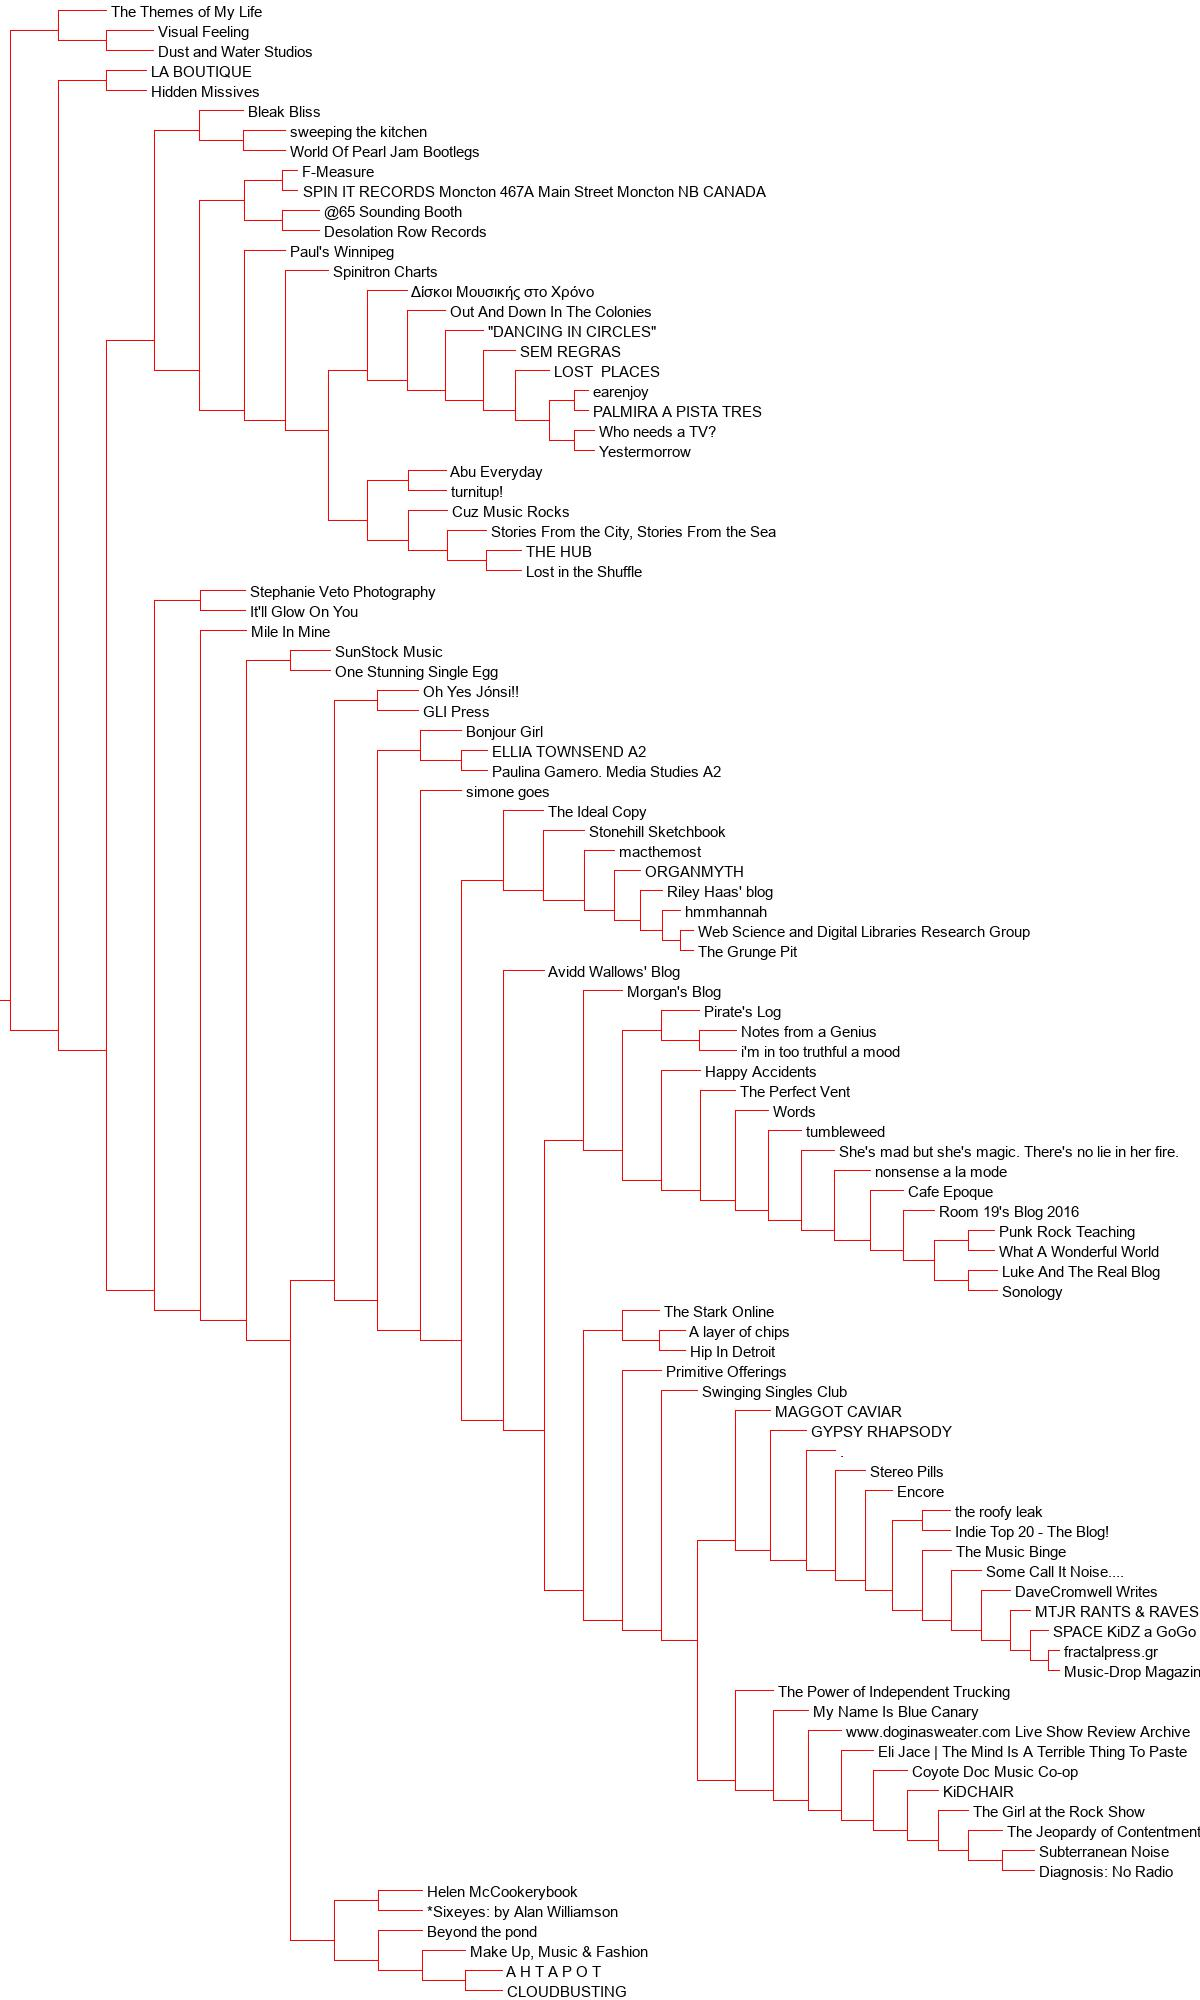
\includegraphics[width=\textwidth, height=0.95\textheight, keepaspectratio]{1blogclust}
\label{dendrogram1}
\end{figure}

\begin{MyPython}[caption=Q2 ClusterImage.py, label=lst:clusterimage]
from sevenhtml import *

blognames, words, data=readfile('2blogdata.txt')
clust=hcluster(data)
printclust(clust, labels=blognames)

drawdendrogram(clust, blognames, jpeg='2blogclust.jpg')

print ('Centroid = 5', end='\n')
kclust= kcluster(data, k=5)
for i in range(5):
    print('Cluster %d' % i, *[blognames[x] for x in kclust[i]], sep='\t')

print('Centroid = 10', end='\n')
kclust= kcluster(data, k=10)
for i in range(10):
    print('Cluster %d' % i, *[blognames[x] for x in kclust[i]], sep='\t')

print('Centroid = 20', end='\n')
kclust= kcluster(data, k=20)
for i in range(20):
    print('Cluster %d' % i, *[blognames[x] for x in kclust[i]], sep='\t')

print('2d Coords', end='\n')
coords= scaledown(data)
draw2d(coords, blognames, jpeg='2blog2d.jpg')
\end{MyPython}


\end{answer}

\begin{answer}{3: K-Means}
Question 3: Cluster the blogs using K-Means, using k=5,10,20. (see slide 18). Print the values in each centroid, for each value of k. How many interations were required for each value of k?\\

For this part, the existing functions from P.C.I. were sufficient. The only alteration was in the ``scaledown()" function. when the pearson score is calculated, it is possible to return a 0, which would throw an error when the function calculates the value ``errorterm". To fix this, an if statement was added to check the value of the denominator, else errorterm=0. The results of the K-Means calculation can be found in Listing \ref{lst:kmeans}
\begin{MyBash}[caption=Q3 Results, label=lst:kmeans]
Centroid = 5
Iteration 0
Iteration 1
Iteration 2
Iteration 3
Iteration 4
Cluster 0	F-Measure	SPIN IT RECORDS Moncton 467A Main Street Moncton NB CANADA	Cafe Epoque	ELLIA TOWNSEND A2	.	SunStock Music	Mile In Mine	Luke And The Real Blog	Make Up, Music & Fashion	Swinging Singles Club	Paulina Gamero. Media Studies A2	Sonology	Desolation Row Records	Indie Top 20 - The Blog!	Notes from a Genius	World Of Pearl Jam Bootlegs	The Perfect Vent	Stereo Pills

Cluster 1	Eli Jace | The Mind Is A Terrible Thing To Paste	Some Call It Noise....	www.doginasweater.com Live Show Review Archive	Coyote Doc Music Co-op	GYPSY RHAPSODY	fractalpress.gr	Primitive Offerings	Helen McCookerybook	Morgan's Blog	The Music Binge	Encore	Paul's Winnipeg	The Jeopardy of Contentment	A layer of chips	Cuz Music Rocks	the roofy leak	Music-Drop Magazine	My Name Is Blue Canary	KiDCHAIR	The Power of Independent Trucking	SPACE KiDZ a GoGo	Subterranean Noise	Diagnosis: No Radio	A H T A P O T	DaveCromwell Writes	The Girl at the Rock Show	?????? ???????? ??? ?????	Abu Everyday	Spinitron Charts	Bonjour Girl	The Themes of My Life	Hip In Detroit	i'm in too truthful a mood	MTJR RANTS & RAVES ON MUSICThe Stark Online	turnitup!	Pirate's Log	Dust and Water Studios	Bleak Bliss	MAGGOT CAVIAR

Cluster 2	Beyond the pond	Who needs a TV?	earenjoy	"DANCING IN CIRCLES"	LOST  PLACES	Stories From the City, Stories From the Sea	sweeping the kitchen	Words	PALMIRA A PISTA TRES	simone goes	Yestermorrow	@65 Sounding Booth	Happy Accidents	Hidden Missives	Visual Feeling	One Stunning Single Egg	CLOUDBUSTING	Out And Down In The Colonies	Lost in the Shuffle	SEM REGRAS	*Sixeyes: by Alan Williamson	It'll Glow On You

Cluster 3	macthemost	hmmhannah	Stonehill Sketchbook	ORGANMYTH	Riley Haas' blog	The Grunge Pit

Cluster 4	Web Science and Digital Libraries Research Group	The Ideal Copy	Stephanie Veto Photography	tumbleweed	Room 19's Blog 2016	THE HUB	She's mad but she's magic. There's no lie in her fire.	Oh Yes J�nsi!!	Punk Rock Teaching	GLI Press	Avidd Wallows' Blog	nonsense a la mode	What A Wonderful World	LA BOUTIQUE

Centroid = 10
Iteration 0
Iteration 1
Iteration 2
Iteration 3
Iteration 4
Iteration 5
Iteration 6
Cluster 0	The Ideal Copy	THE HUB	Punk Rock Teaching	LA BOUTIQUE	Lost in the Shuffle

Cluster 1	GYPSY RHAPSODY	The Music Binge	Encore	.	SunStock Music	the roofy leak	Swinging Singles Club	Indie Top 20 - The Blog!	The Stark Online	*Sixeyes: by Alan Williamson	Dust and Water Studios	MAGGOT CAVIAR	Stereo Pills

Cluster 2	Stories From the City, Stories From the Sea	Paul's Winnipeg	Cuz Music Rocks	A H T A P O T	@65 Sounding Booth	GLI Press	CLOUDBUSTING

Cluster 3	Web Science and Digital Libraries Research Group	macthemost	Stonehill Sketchbook	ORGANMYTH	Riley Haas' blog	The Grunge Pit

Cluster 4	Stephanie Veto Photography	hmmhannah	Oh Yes J�nsi!!	nonsense a la mode	The Perfect Vent	It'll Glow On You

Cluster 5	Who needs a TV?	earenjoy	Primitive Offerings	"DANCING IN CIRCLESLOST  PLACES	sweeping the kitchen	PALMIRA A PISTA TRES	Mile In Mine	YestermorroA layer of chips	Avidd Wallows' Blog	Hidden Missives	Visual Feeling	Hip In Detroit	SEM REGRAS	Bleak Bliss

Cluster 6	Eli Jace | The Mind Is A Terrible Thing To Paste	Some Call It Noise....	www.doginasweater.com Live Show Review Archive	Coyote Doc Music Co-op	simone goesThe Jeopardy of Contentment	My Name Is Blue Canary	KiDCHAIR	The Power of Independent Trucking	Subterranean Noise	Diagnosis: No Radio	DaveCromwell Writes	The Girl at the Rock Show	Paulina Gamero. Media Studies A2	Abu Everyday	Bonjour GirNotes from a Genius	i'm in too truthful a mood

Cluster 7	F-Measure	fractalpress.gr	SPIN IT RECORDS Moncton 467A Main Street Moncton NB CANADA	ELLIA TOWNSEND A2	Music-Drop Magazine	SPACE KiDZ a GoGo	?????? ???????? ??? ?????	Spinitron Charts	Out And Down In The Colonies	Desolation Row Records	The Themes of My Life	World Of Pearl Jam Bootlegs	MTJR RANTS & RAVES ON MUSIC	turnitup!

Cluster 8	Beyond the pond	tumbleweed	Room 19's Blog 2016	Helen McCookerybookMorgan's Blog	Words	Cafe Epoque	She's mad but she's magic. There's no lie in her fire.	Luke And The Real Blog	Make Up, Music & Fashion	What A Wonderful World	Happy Accidents	Sonology	One Stunning Single Egg	Pirate's Log

Cluster 9

Centroid = 20
Iteration 0
Iteration 1
Iteration 2
Iteration 3
Iteration 4
Iteration 5
Iteration 6
Iteration 7
Iteration 8
Iteration 9
Iteration 10
Iteration 11
Iteration 12
Iteration 13
Cluster 0
Cluster 1	PALMIRA A PISTA TRES	simone goes	hmmhannah	Oh Yes J�nsi!!	It'll Glow On You

Cluster 2	The Grunge Pit

Cluster 3	Some Call It Noise....	www.doginasweater.com Live Show Review Archive	Coyote Doc Music Co-op	GYPSY RHAPSODY	Primitive Offerings	The Music Binge	Encore	Paul's Winnipeg	The Jeopardy of Contentment	A layer of chips	the roofy leak	My Name Is Blue Canary	KiDCHAIR	The Power of Independent Trucking	Subterranean Noise	Diagnosis: No Radio	DaveCromwell Writes	The Girl at the Rock Show	Swinging Singles Club	Bonjour Girl	The Stark Online	*Sixeyes: by Alan WilliamsoDust and Water Studios

Cluster 4

Cluster 5	LOST  PLACES	LA BOUTIQUE	Hidden Missives	SEM REGRAS

Cluster 6	The Ideal Copy	Happy Accidents

Cluster 7	Riley Haas' blog

Cluster 8	Beyond the pond	Helen McCookerybook	THE HUB	Cafe Epoque	Lost in the Shuffle

Cluster 9	Stonehill Sketchbook	ORGANMYTH

Cluster 10	Who needs a TV?	earenjoy	tumbleweed	"DANCING IN CIRCLES"	Words	She's mad but she's magic. There's no lie in her fire.	Mile In Mine	YestermorroAvidd Wallows' Blog	nonsense a la mode	Visual Feeling

Cluster 11	Morgan's Blog	Luke And The Real Blog	Punk Rock Teaching	What A Wonderful World	Sonology	Notes from a Genius	The Perfect Vent	i'm in too truthful a mood	Pirate's Log

Cluster 12

Cluster 13	Web Science and Digital Libraries Research Group	Stories From the City, Stories From the Sea	Make Up, Music & Fashion	GLI Press	Paulina Gamero. Media Studies A2	CLOUDBUSTING	Hip In Detroit

Cluster 14	Room 19's Blog 2016	Bleak Bliss	MAGGOT CAVIAR

Cluster 15

Cluster 16	fractalpress.gr	ELLIA TOWNSEND A2	Music-Drop Magazine	SPACE KiDZ a GoGo	A H T A P O T	?????? ???????? ??? ?????	Spinitron Charts	Out And Down In The Colonies	The Themes of My Life	MTJR RANTS & RAVES ON MUSIC	turnitup!

Cluster 17	F-Measure	SPIN IT RECORDS Moncton 467A Main Street Moncton NB CANADA	SunStock Music	@65 Sounding Booth	Desolation Row Records	Indie Top 20 - The Blog!	World Of Pearl Jam Bootlegs	Stereo Pills

Cluster 18	macthemost

Cluster 19	Eli Jace | The Mind Is A Terrible Thing To Paste	Stephanie Veto Photography	sweeping the kitchen	Cuz Music Rocks	Abu Everyday	One Stunning Single Egg
\end{MyBash}

\end{answer}

\begin{answer}{4: MultiDimensional Scaling}
Use MDS to create a JPEG of the blogs similar to slide 29 of the
week 12 lecture. How many iterations were required?\\
The example from P.C.I worked just fine for this portion. The only issue was once again, the font had to be declared and passed to ``draw.text(font=font)". The functions can be found in Listing \ref{lst:sevenhtml} and the resulting jpeg in Figure \ref{1blog2d} with 316 iterations.
\FloatBarrier
\begin{figure}
\caption{Q4 2D MDS}
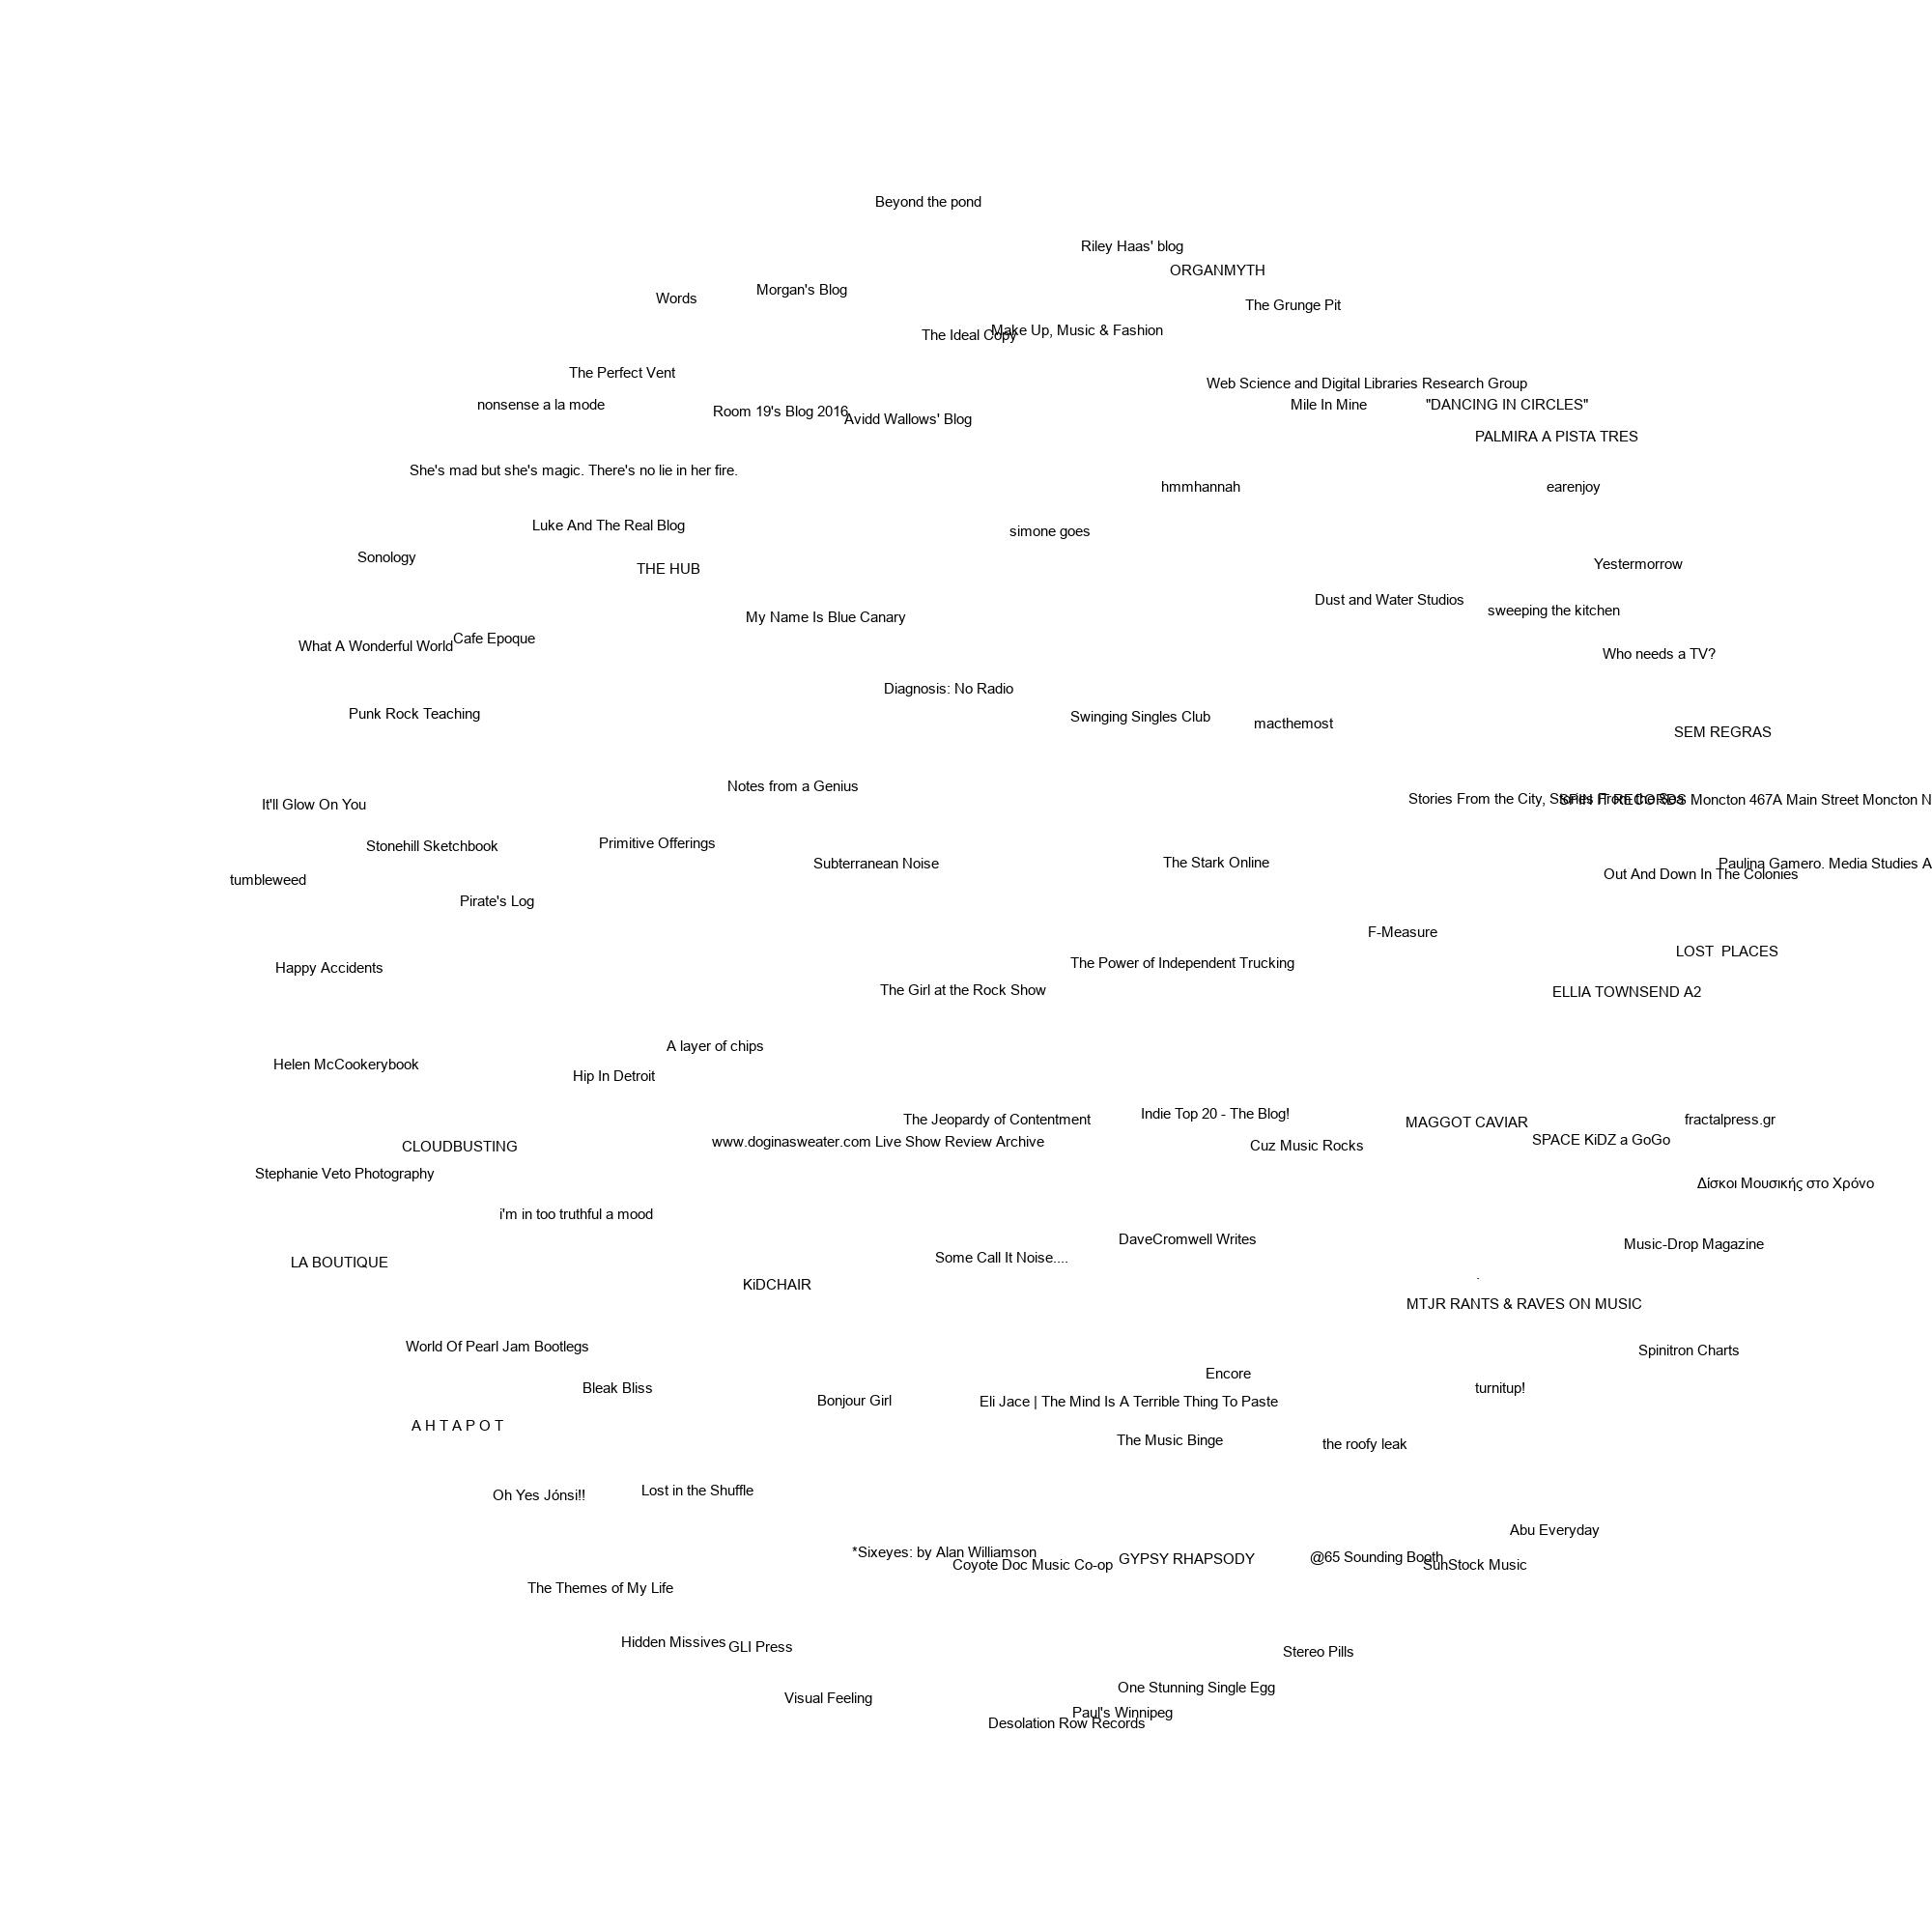
\includegraphics[width=\textwidth, height=0.95\textheight , keepaspectratio]{1blog2d}
\label{1blog2d}
\end{figure}
\FloatBarrier
\end{answer}

\begin{answer}{5: Re-Run Question 2}
Question 5: Re-run question 2, but this time with proper TFIDF calculations instead of the hack discussed on slide 7 (p. 32). Use the same 1000 words, but this time replace their frequency count with TFIDF scores as computed in assignment 3. Document the code, techniques, methods, etc. used to generate these TFIDF values. Upload the new data file to github. Compare and contrast the resulting dendrogram with the dendrogram from question 2. Note: ideally you would not reuse the same 1000 terms and instead come up with TFIDF scores for all the terms and then choose the top 1000 from that list, but I'm trying to limit the amount of work necessary.\\

This part did not require a huge change. All of the inormation was already there. The updated code is shown in Listing \ref{lst:generatefeedvector} surrounded by hash lines. I also had to change the print to file portion to print floats instead of digits. The dendrogram shown in Figure \ref{dendrogram2} is similar in shape to Figure \ref{dendrogram1} from Question 2. In both there are two main branches that split close to the left side, and then branch further from there. the main difference is that in Figure \ref{dendrogram2} the branches are more evenly divided, while in Figure \ref{dendrogram1} most of the blogs are on the lower branch. Other than that, the blogs tend to be similarly grouped. ``Punk Rock Teaching" is still next to ``What a Wonderful World" and ``Lost in the Shuffle" is still next to ``The Hub" and ``Stories from the City".
\FloatBarrier
\begin{figure}
\caption{Q5 Dendrogram}
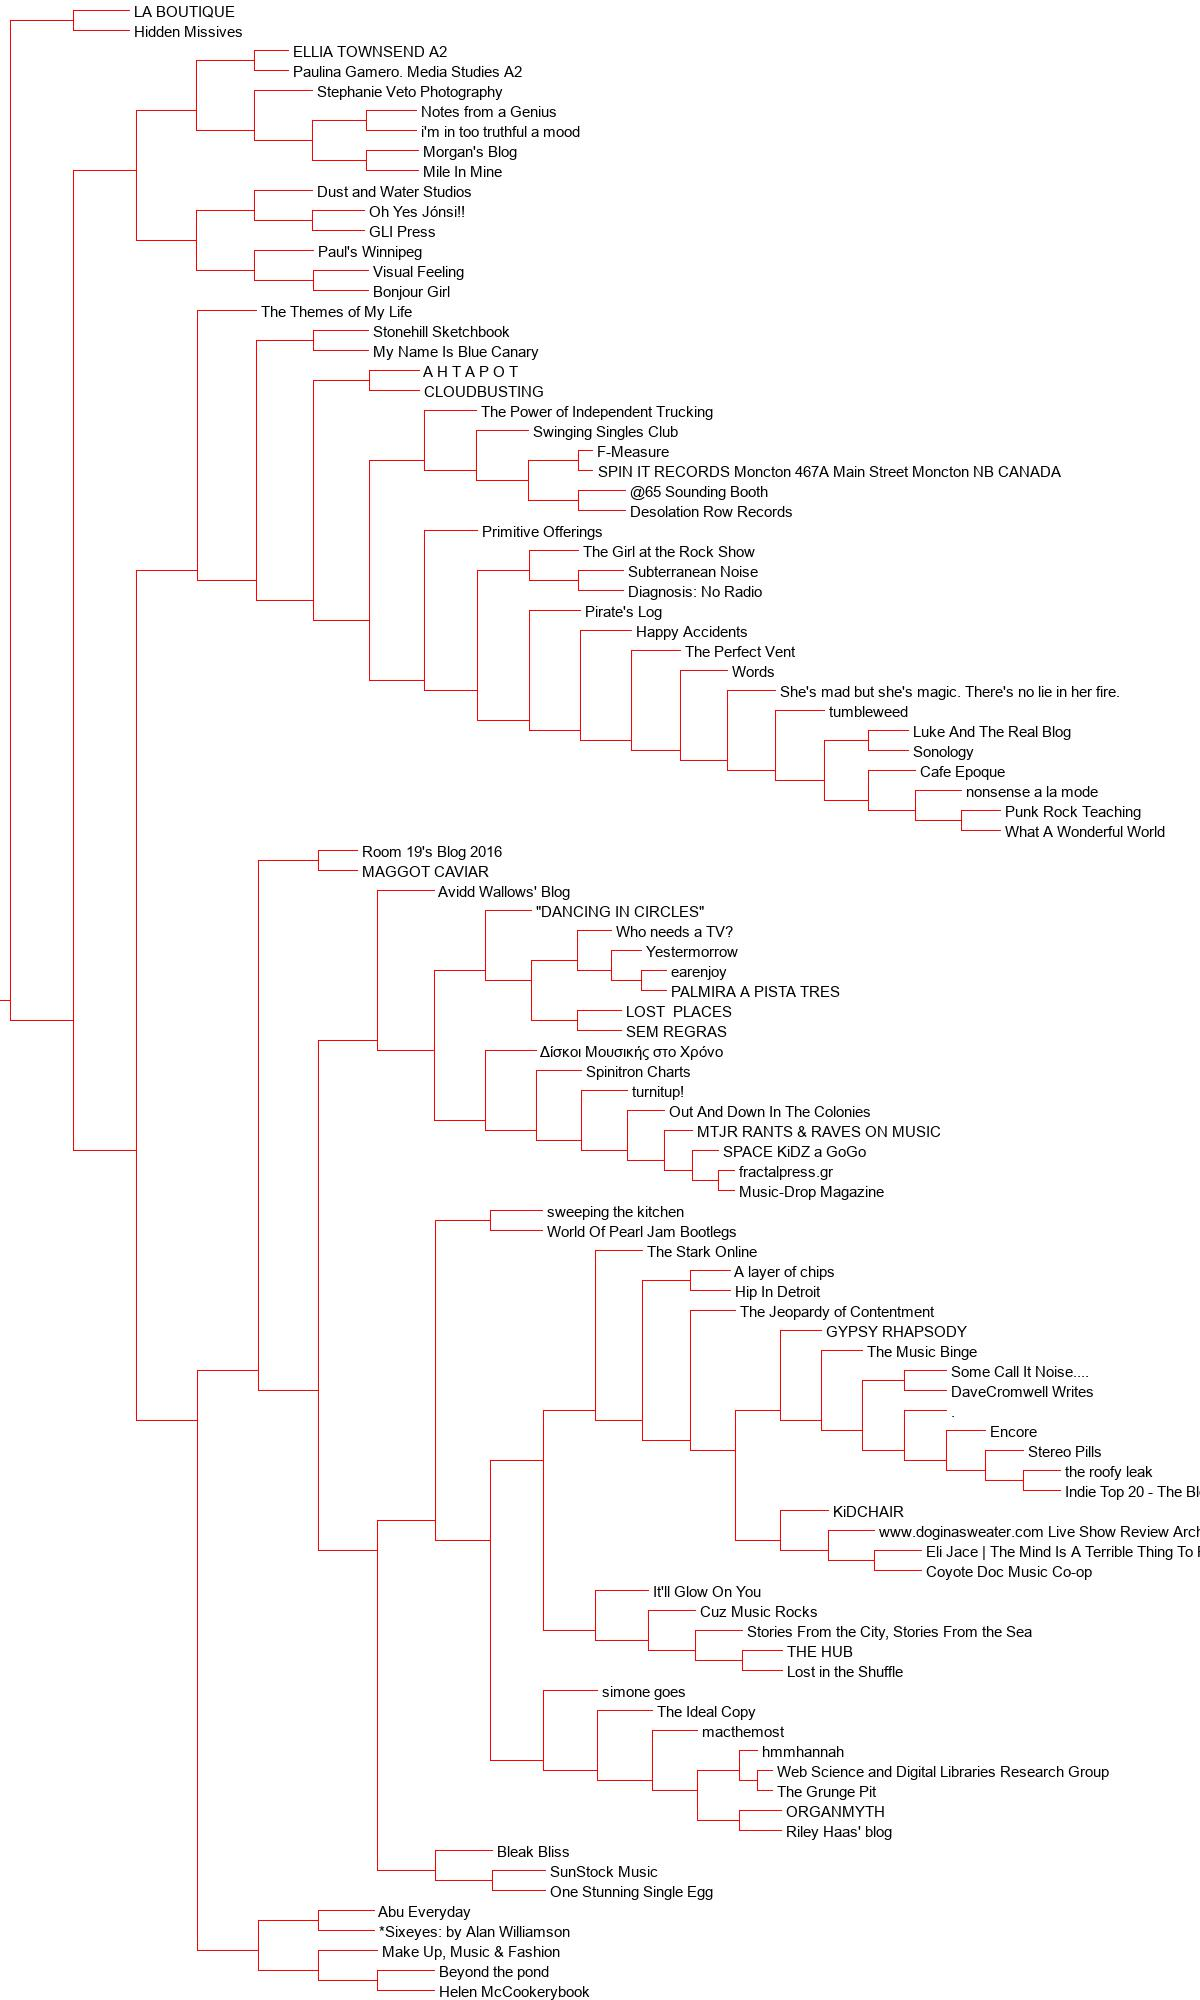
\includegraphics[width=\textwidth, height=0.95\textheight , keepaspectratio]{2blogclust}
\label{dendrogram2}
\end{figure}
\FloatBarrier
\end{answer}

\begin{MyPython}[caption=Generate Feed Vector, label=lst:generatefeedvector]
from sevenhtml import *
from math import log2, log10, floor
import sys

round_to_n=lambda x, n: round(x, -int(floor(log10(abs(x))))+(n-1))
apcount={}
wordcounts={}
for feedurl in open('lurl.txt'):
    try:
        (title, wc)=getwordcounts(feedurl)
    except KeyError:
        sys.stdout.write('Key Error on %s' % feedurl)
        continue
    sys.stdout.write('\r%d URL: %s'% (len(wordcounts), feedurl))
    sys.stdout.flush()
    wordcounts[title]=wc
    for word,count in wc.items( ):
        apcount.setdefault(word,0)
        apcount[word]+=1
    if len(wordcounts)==100:
        break

wordtuple=[]
for w,bc in apcount.items( ):
    frac=float(bc)/len(wordcounts)
    if frac>0.1 and frac<0.5:
        wordtuple.append((w, frac))
wordtuple.sort(key=lambda x: x[1], reverse=True)
wordlist=list(x[0] for x in wordtuple)
if len(wordlist)>1000:
    del wordlist[1000:]
print('Number of Words: %d' % len(wordlist))
print(*wordlist, sep='\n')
del wordtuple

#this section is added for TFIDF scores
#|||||||||||||||||||||||||||||||||||||
for blog,wc in wordcounts.items():
    totalwords=sum(wc.values())
    for word in wordlist:
        if word in wc:
            wc[word]=(wc[word]/float(totalwords))*(log2(len(wordcounts)/float(apcount[word])))
#|||||||||||||||||||||||||||||||||||||
out=open('2blogdata.txt','w')
out.write('Blog')

for word in wordlist:
    out.write('\t%s' %word)
out.write('\n')
for blog, wc in wordcounts.items():
    out.write(blog)
    for word in wordlist:
        if word in wc:
        	    #this part was changed from %d to %f to deal with the floats in TFIDF
            out.write('\t%f' % wc[word])
        else:
            out.write('\t0')
    out.write('\n')
\end{MyPython}

\begin{MyPython}[caption= sevenhtml, label=lst:sevenhtml]
import requests
import feedparser
import re
from bs4 import BeautifulSoup as bs
from math import sqrt
from PIL import Image, ImageDraw, ImageFont
import random

def pull_page(address):
    address=address.rstrip()
    header={'User-Agent': 'Mozilla/5.0 (Macintosh; Intel Mac OS X 10_12_3) AppleWebKit/537.36 (KHTML, like Gecko) Chrome/56.0.2924.87 Safari/537.36'}
    tpage=requests.get(address, headers=header, allow_redirects=True)
    return tpage

def get_random_blog(language):
    address='http://www.blogger.com/next-blog?navBar=true&blogID=3471633091411211117'
    header={'User-Agent': 'Mozilla/5.0 (Macintosh; Intel Mac OS X 10_12_3) AppleWebKit/537.36 (KHTML, like Gecko) Chrome/56.0.2924.87 Safari/537.36', 'Accept-Language':'en'}
    while True:
        tpage=requests.get(address, headers=header, allow_redirects=True, stream=True)
        taddy=tpage.url.rstrip('?expref=next-blog')
        spage=requests.get(taddy, headers=header, allow_redirects=True, stream=True)
        soup=bs(spage.text, 'lxml')
        link=soup.find('link', type='application/rss+xml')
        if link is not None:
            return link['href']

# Returns title and dictionary of word counts for an RSS feed
def getwordcounts(url):
    # Parse the feed
    header={'User-Agent': 'Mozilla/5.0 (Macintosh; Intel Mac OS X 10_12_3) AppleWebKit/537.36 (KHTML, like Gecko) Chrome/56.0.2924.87 Safari/537.36', 'Accept-Language':'en'}
    wc={}
    while True:
        d=feedparser.parse(url)
        # Loop over all the entries
        for e in d.entries:
            if 'summary' in e:
                summary=e.summary
            else:
                summary=e.description
            # Extract a list of words
            words=getwords(e.title+' '+summary)
            for word in words:
                wc.setdefault(word,0)
                wc[word]+=1
        tpage=requests.get(url, headers=header, allow_redirects=True, stream=True)
        soup=bs(tpage.text, 'lxml')
        link=soup.find('link', rel='next', type='application/rss+xml')
        if link is not None:
            try:
                url=link['href']
                continue
            except:
                break
        else: break
    
    return d['feed']['title'],wc

def getwords(html):
    # Remove all the HTML tags
    txt=re.compile(r'<[^>]+>').sub('',html)
    # Split words by all non-alpha characters
    words=re.compile(r'[^A-Z^a-z]+').split(txt)
    # Convert to lowercase
    return [word.lower( ) for word in words if word!='']

def readfile(filename):
    lines=[line for line in open(filename, 'r')]
    # First line is the column titles
    colnames=lines[0].strip( ).split('\t')[1:]
    rownames=[]
    data=[]
    for line in lines[1:]:
        p=line.strip( ).split('\t')
        # First column in each row is the rowname
        rownames.append(p[0])
        # The data for this row is the remainder of the row
        data.append([float(x) for x in p[1:]])
    return rownames,colnames,data

def pearson(v1,v2):
    # Simple sums
    sum1=sum(v1)
    sum2=sum(v2)
    # Sums of the squares
    sum1Sq=sum([pow(v,2) for v in v1])
    sum2Sq=sum([pow(v,2) for v in v2])
    # Sum of the products
    pSum=sum([v1[i]*v2[i] for i in range(len(v1))])
    # Calculate r (Pearson score)
    num=pSum-(sum1*sum2/len(v1))
    den=sqrt((sum1Sq-pow(sum1,2)/len(v1))*(sum2Sq-pow(sum2,2)/len(v1)))
    if den==0:
        return 0
    return 1.0-num/den

class bicluster:
    def __init__(self,vec,left=None,right=None,distance=0.0,id=None):
        self.left=left
        self.right=right
        self.vec=vec
        self.id=id
        self.distance=distance

def hcluster(rows,distance=pearson):
    distances={}
    currentclustid=-1
    # Clusters are initially just the rows
    clust=[bicluster(rows[i],id=i) for i in range(len(rows))]
    while len(clust)>1:
        lowestpair=(0,1)
        closest=distance(clust[0].vec,clust[1].vec)
        # loop through every pair looking for the smallest distance
        for i in range(len(clust)):
            for j in range(i+1,len(clust)):
                # distances is the cache of distance calculations
                if (clust[i].id,clust[j].id) not in distances:
                    distances[(clust[i].id,clust[j].id)]=distance(clust[i].vec,clust[j].vec)
                d=distances[(clust[i].id,clust[j].id)]
                if d<closest:
                    closest=d
                    lowestpair=(i,j)
        # calculate the average of the two clusters
        mergevec=[(clust[lowestpair[0]].vec[i]+clust[lowestpair[1]].vec[i])/2.0 for i in range(len(clust[0].vec))]
        # create the new cluster
        newcluster=bicluster(mergevec,left=clust[lowestpair[0]], right=clust[lowestpair[1]], distance=closest,id=currentclustid)
        # cluster ids that weren't in the original set are negative
        currentclustid-=1
        del clust[lowestpair[1]]
        del clust[lowestpair[0]]
        clust.append(newcluster)
    return clust[0]

def printclust(clust,labels=None,n=0):
    # indent to make a hierarchy layout
    for i in range(n):
        print (' ', end='')
    if clust.id<0:
        # negative id means that this is branch
        print ('-')
    else:
        # positive id means that this is an endpoint
        if labels==None:
            print (clust.id)
        else:
            print (labels[clust.id])
    # now print the right and left branches
    if clust.left!=None:
        printclust(clust.left,labels=labels,n=n+1)
    if clust.right!=None:
        printclust(clust.right,labels=labels,n=n+1)

def getheight(clust):
    # Is this an endpoint? Then the height is just 1
    if clust.left==None and clust.right==None:
        return 1
    # Otherwise the height is the same of the heights of
    # each branch
    return getheight(clust.left)+getheight(clust.right)

def getdepth(clust):
    # The distance of an endpoint is 0.0
    if clust.left==None and clust.right==None: return 0
    # The distance of a branch is the greater of its two sides
    # plus its own distance
    return max(getdepth(clust.left),getdepth(clust.right))+clust.distance

def drawdendrogram(clust,labels,jpeg='clusters.jpg'):
    font=ImageFont.truetype('arial.ttf', 15)
    # height and width
    h=getheight(clust)*20
    w=1200
    depth=getdepth(clust)
    # width is fixed, so scale distances accordingly
    if depth is not 0:
        scaling=float(w-150)/depth
    else: scaling=0
    # Create a new image with a white background
    img=Image.new('RGB',(w,h),(255,255,255))
    draw=ImageDraw.Draw(img)
    draw.line((0,h/2,10,h/2),fill=(255,0,0))
    # Draw the first node
    drawnode(draw,clust,10,(h/2),scaling,labels, font=font)
    img.save(jpeg,'JPEG')

def drawnode(draw,clust,x,y,scaling,labels, font=None):
    if clust.id<0:
        h1=getheight(clust.left)*20
        h2=getheight(clust.right)*20
        top=y-(h1+h2)/2
        bottom=y+(h1+h2)/2
        # Line length
        ll=clust.distance*scaling
        # Vertical line from this cluster to children
        draw.line((x,top+h1/2,x,bottom-h2/2),fill=(255,0,0))
        # Horizontal line to left item
        draw.line((x,top+h1/2,x+ll,top+h1/2),fill=(255,0,0))
        # Horizontal line to right item
        draw.line((x,bottom-h2/2,x+ll,bottom-h2/2),fill=(255,0,0))
        # Call the function to draw the left and right nodes
        drawnode(draw,clust.left,x+ll,top+h1/2,scaling,labels, font=font)
        drawnode(draw,clust.right,x+ll,bottom-h2/2,scaling,labels, font=font)
    else:
        # If this is an endpoint, draw the item label
        draw.text((x+5,y-7),labels[clust.id],(0,0,0), font=font)

def rotatematrix(data):
    newdata=[]
    for i in range(len(data[0])):
        newrow=[data[j][i] for j in range(len(data))]
        newdata.append(newrow)
    return newdata

def kcluster(rows,distance=pearson,k=4):
    # Determine the minimum and maximum values for each point
    ranges=[(min([row[i] for row in rows]),max([row[i] for row in rows])) for i in range(len(rows[0]))]
    # Create k randomly placed centroids
    clusters=[[random.random( )*(ranges[i][1]-ranges[i][0])+ranges[i][0] for i in range(len(rows[0]))] for j in range(k)]
    lastmatches=None
    for t in range(100):
        print ('Iteration %d' % t)
        bestmatches=[[] for i in range(k)]
        # Find which centroid is the closest for each row
        for j in range(len(rows)):
            row=rows[j]
            bestmatch=0
            for i in range(k):
                d=distance(clusters[i],row)
                if d<distance(clusters[bestmatch],row):
                    bestmatch=i
            bestmatches[bestmatch].append(j)
        # If the results are the same as last time, this is complete
        if bestmatches==lastmatches:
            break
        lastmatches=bestmatches
        # Move the centroids to the average of their members
        for i in range(k):
            avgs=[0.0]*len(rows[0])
            if len(bestmatches[i])>0:
                for rowid in bestmatches[i]:
                    for m in range(len(rows[rowid])):
                        avgs[m]+=rows[rowid][m]
                for j in range(len(avgs)):
                    avgs[j]/=len(bestmatches[i])
                clusters[i]=avgs
    return bestmatches

def scaledown(data,distance=pearson,rate=0.01):
    n=len(data)
    iteration=0
    # The real distances between every pair of items
    realdist=[[distance(data[i],data[j]) for j in range(n)] for i in range(0,n)]
    outersum=0.0
    # Randomly initialize the starting points of the locations in 2D
    loc=[[random.random(),random.random( )] for i in range(n)]
    fakedist=[[0.0 for j in range(n)] for i in range(n)]
    lasterror=None
    for m in range(0,1000):
        # Find projected distances
        for i in range(n):
            for j in range(n):
                fakedist[i][j]=sqrt(sum([pow(loc[i][x]-loc[j][x],2) for x in range(len(loc[i]))]))
        # Move points
        grad=[[0.0,0.0]for i in range(n)]
        totalerror=0
        for k in range(n):
            for j in range(n):
                if j==k:
                    continue
                # The error is percent difference between the distances

                errorterm=0
                if realdist[j][k]>0:
                    errorterm=(fakedist[j][k]-realdist[j][k])/realdist[j][k]
                # Each point needs to be moved away from or towards the other
                # point in proportion to how much error it has
                grad[k][0]+=((loc[k][0]-loc[j][0])/fakedist[j][k])*errorterm
                grad[k][1]+=((loc[k][1]-loc[j][1])/fakedist[j][k])*errorterm
                # Keep track of the total error
                totalerror+=abs(errorterm)
        print (totalerror)
        iteration+=1
        # If the answer got worse by moving the points, we are done
        if lasterror and lasterror<totalerror: break
        lasterror=totalerror
        # Move each of the points by the learning rate times the gradient
        for k in range(n):
            loc[k][0]-=rate*grad[k][0]
            loc[k][1]-=rate*grad[k][1]
    print(iteration)
    return loc

def draw2d(data,labels,jpeg='mds2d.jpg'):
    font=ImageFont.truetype('arial.ttf', 15)
    img=Image.new('RGB',(2000,2000),(255,255,255))
    draw=ImageDraw.Draw(img)
    for i in range(len(data)):
        x=(data[i][0]+0.5)*1000
        y=(data[i][1]+0.5)*1000
        draw.text((x,y),labels[i],(0,0,0), font=font)
    img.save(jpeg,'JPEG')
\end{MyPython}

\begin{alltt}
\input{lurl.txt}
\end{alltt}



\end{document}